%%
%% The official i6 slide template _demo_
%% created by Philippe Dreuw and Thomas Deselaers, 2005
%%
%% $Id: slides.tex,v 1.50 2008-07-17 09:21:35 dreuw Exp $
%%
%% Possible options for:
%%  - language       : 'english' (default), 'german'
%%  - page numbering : 'nonumber', 'lastpage' to enable automatic page n/m numbering, 
%%                     'userlastpage' to enable a user defined page n/m numbering using \LastPage command,  
%%                      or leave empty for normal page numbering (default)
%%  - itemize        : 'triangle' or leave empty for bullets (default)
%%  - page layout    : 'vertical' to enable vertical centering on each slide using \vfill ... \vfill (default)
%%                     'demo' to compile images in demo mode, i.e. image files are not necessary 
%%  - encoding       : 'utf-8' to enable utf encoding instead of latin1 (default)
%%  - tools          : 'noblackslide' to disable the black slide at the end which is linked with every slide title, e.g. to write a proof on the blackboard
%%
\documentclass[11pt, a4paper, landscape]{article}
%\usepackage[userlastpage,triangle,demo]{NeyDreuwSlides_Oct08}  % if you don't have the images
\usepackage[userlastpage,triangle,utf-8]{NeyDreuwSlides_Oct08}  % if you don't have the images
\usepackage{snapshot} 
\usepackage{float}
\usepackage{lastpage}

% slides tunning
%\setlength{\footskip}{0pt}       % default ist +30pt - negative Werte nicht moeglich
%\setlength{\headsep}{-10pt}      % default ist +25pt - negative Werte moeglich
%\addtolength{\topmargin}{-5mm}   % bewegt den gesamten Inhalt der Seite nach oben
%\setlength{\textheight}{170mm}   % wenn moeglich nicht veraendern, beinflusst den Inhalt der Seiten und somit auch die Anzahl der Seiten!



% math operators and symbols %%%%%%%%%%%%%%%%%%%%%%%%%%%%%%%%%%%%%%%%%%%%%%%%%%%
\newcommand*{\nat}{\ensuremath{\rm I\!N}\xspace}
\newcommand*{\rel}{\ensuremath{\rm I\!R}\xspace}
\newcommand*{\argmin}{\ensuremath{\operatornamewithlimits{argmin}}\xspace}
\newcommand*{\argmax}{\ensuremath{\operatornamewithlimits{argmax}}\xspace}
\newcommand*{\congmod}{\ensuremath{\operatornamewithlimits{\cong}}\xspace}
\newcommand*{\invers}{\ensuremath{\frac{1}}\xspace}
\newcommand*{\ra}{\ensuremath{\Rightarrow}\xspace}


%%%%%%%%%%%%%%%%%%%%%%%%%%%%%%%%%%%%%%%%%%%%%%%%%%%%%%%%%%%%%%%%%%%%%%%%%%%%%%%%
%% flyspell can read the local ispelldict variable to automatically change the dictionary, 
%% e.g. german-new8, american, english, british, ...
%% 
%% Local IspellDict: american
%% 


%%%%%%%%%%%%%%%%%%%%%%%%%%%%%%%%%%%%%%%%%%%%%%%%%%%%%%%%%%%%%%%%%%%%%%%%%%%%%%%%
% custom packages
\usepackage{fancyvrb} %%% fancy verbatim to enable coloring within verbatim environments
%\usepackage{pst-node} 
%\usepackage[encapsulated]{CJK}
%\newcommand{\cjs}[1]{\begin{CJK}{UTF8}{gbsn}#1\end{CJK}}
%\usepackage{CJK}
%\usepackage{arabtex}   
%\novocalize


%%%%%%%%%%%%%%%%%%%%%%%%%%%%%%%%%%%%%%%%%%%%%%%%%%%%%%%%%%%%%%%%%%%%%%%%%%%%%%%%
% Some example hacks work only in combination with the 'pdflatex -shell-escape'
% mode. Try 'make hacks'


%%%%%%%%%%%%%%%%%%%%%%%%%%%%%%%%%%%%%%%%%%%%%%%%%%%%%%%%%%%%%%%%%%%%%%%%%%%%%%%%
\renewcommand*{\title}{Character-based Embeddings of Words with Recurrent~Nets}        % main title of the work (used for \TitlePage)
\renewcommand*{\titleshort}{ Word Embeddings RNN}                                 % short title (used for \lfoot)
\renewcommand*{\occasion}{Seminar Selected Topics in Human Language Technology and Pattern Recognition}%     % (used for \TitlePage) 
\renewcommand*{\occasionshort}{Selected Topics Human Language Technology}               % short occasion title (used for \rfoot)
%\renewcommand*{\date}{11. April 2005}                                        % default is \today (used for \TitlePage and \rfoot)
\renewcommand*{\author}{Simon Gr\"atzer}         % all the authors of the work, can be long (used for \TitlePage)
\renewcommand*{\authorshort}{S. Gr\"atzer}                            % all the authors of the work, should be short (used for \lfoot)
%\renewcommand*{\email}{\url{{deselaers,dreuw}@i6.informatik.rwth-aachen.de}}  % all email address(es) of the authors (used for \TitlePage)
\renewcommand*{\mainauthor}{Simon Grätzer}                                   % the author(s) who presented the work (used for \TitlePage)
\renewcommand*{\mainauthoremail}{\url{simon.graetzer@rwth-aachen.de}}    % presenter mail address(es) (used for \FinalPage)
\renewcommand*{\www}{http://www-i6.informatik.rwth-aachen.de/}                % web address (used for \TitlePage _and_ \FinalPage)
\newcommand*{\keywords}{Word Embeddings, LSTM, Language Modeling}                               % keywords, can be used for PDF summary

% will be set into the PDF document summary
\hypersetup{
  pdftitle={\title}, 
  pdfsubject={\occasion},  
  pdfauthor={\author}, 
  pdfkeywords={\keywords},
  % enable automatic page transitions: for endless loop edit in
  % acrobat reader -> preferences -> full screen -> after every X
  % seconds and after last page
  pdfpageduration = 2, 
%  pdfpagetransition = {Glitter /Di 315 /D 5}  
  pdfpagetransition = {Box /M /O /D 1},
}

%%%%%%%%%%%%%%%%%%%%%%%%%%%%%%%%%%%%%%%%%%%%%%%%%%%%%%%%%%%%%%%%%%%%%%%%%%%%%%%%
\listfiles
%%%%%%%%%%%%%%%%%%%%%%%%%%%%%%%%%%%%%%%%%%%%%%%%%%%%%%%%%%%%%%%%%%%%%%%%%%%%%%%%
\begin{document}
%%%%%%%%%%%%%%%%%%%%%%%%%%%%%%%%%%%%%%%%%%%%%%%%%%%%%%%%%%%%%%%%%%%%%%%%%%%%%%%%
\TitlePage

%%%%%%%%%%%%%%%%%%%%%%%%%%%%%%%%%%%%%%%%%%%%%%%%%%%%%%%%%%%%%%%%%%%%%%%%%%%%%%%%
\NewPage\headline{Outline}
\small
\vfill
\begin{enumerate}
\item \hyperlink{sli:introduction}{Introduction}
\item \hyperlink{sli:word-embeddings}{Word Embeddings}
\begin{enumerate}
\item \hyperlink{sli:goals}{Goals}
\item \hyperlink{sli:simple}{Continuous Space Language Model}
\item Shortcomings of Word Lookup Tables
\end{enumerate}
\item Character-based Word-Embeddings
\item Experimentation
\begin{enumerate}
\item Language Modeling
\item Part-Of-Speech Tagging
\item Morphological Inflection Generation
\end{enumerate}

%\item[] \hyperlink{sli:bibliography}{Bibliography}
%\item[] \hyperlink{sli:appendix}{Appendix}
\end{enumerate}
\vfill
\normalsize
\vfill

%%%%%%%%%%%%%%%%%%%%%%%%%%%%%%%%%%%%%%%%%%%%%%%%%%%%%%%%%%%%%%%%%%%%%%%%%%%%%%%%
\NewPage\headline{Literature} 
\vfill
\begin{description}

\item [Wang Ling et al 2015 :] Finding Function in Form: Compositional Character Models for Open 
      Vocabulary Word Representation. CoRR Volume abs/1508.02096, 2015 
  \begin{itemize}
  \item Introduces a model for constructing vector representations of words by composing characters using bidirectional LSTMs.
  \end{itemize}

\item [Faruqui et al 2015 :] Morphological Inflection Generation Using Character Sequence to Sequence Learning. CoRR Volume abs/1512.06110, 2015 
  \begin{itemize}
  \item Approach to generate inflected versions of words by modelling the process as a character sequence to sequence learning problem.
  \end{itemize}

\item [Mikolov et al 2013 :] Distributed Representations of Words and Phrases and their Compositionality. CoRR Volume abs/1310.4546, 2013 
  \begin{itemize}
  \item Improvements on the Skip-gram model used to generate word embeddings.
  \end{itemize}

\end{description}
\vfill


%%%%%%%%%%%%%%%%%%%%%%%%%%%%%%%%%%%%%%%%%%%%%%%%%%%%%%%%%%%%%%%%%%%%%%%%%%%%%%%%
\NewPage\headline{Literature} 
\vfill
\begin{description}

\item [Schwenk 2007 :] Continuous Space Language Models. Journal Computer Speech and Language. Volume 21 Issue 3, July, 2007 Pages 492-518 
  \begin{itemize}
  \item Describes the use of a neural network language model for large vocabulary continuous speech recognition.
  \end{itemize}

\item [Peirsman 2015 :] Visualizing Word Embeddings with t-SNE. Online 2015
  \begin{itemize}
  \item Creating useful low-dimensional visualizations for high-dimensional datasets
  \end{itemize}
  
\item [TensorFlow 2016 :] Vector Representations of Words, From the TensorFlow documentation
  \begin{itemize}
  \item Implementation of word2vec model of [Mikolov et al 2013] with the TensorFlow framework.
  \end{itemize}
\end{description}
\vfill


%%%%%%%%%%%%%%%%%%%%%%%%%%%%%%%%%%%%%%%%%%%%%%%%%%%%%%%%%%%%%%%%%%%%%%%%%%%%%%%%
\NewPage\headline{Introduction} 
\hypertarget{sli:introduction}{}

\vfill
\begin{itemize}
\item Word embeddings are real valued vector representations for words.
\item This talk is about generating word embeddings and their applications.
\item Specifically:
  \begin{itemize}
  \item Generating word embeddings by composing their individual character representations
  \item Using Long short-term memory to capture complex relationships between words.
\end{itemize}
\item The resulting model can be used for many tasks, such as language modeling or part-of-speech tagging
\item Reduces the need for manual feature engineering
\item Can improve performance for many tasks
\end{itemize}
\vfill

%%%%%%%%%%%%%%%%%%%%%%%%%%%%%%%%%%%%%%%%%%%%%%%%%%%%%%%%%%%%%%%%%%%%%%%%%%%%%%%%
\NewPage\headline{Introduction} 


\begin{center}
  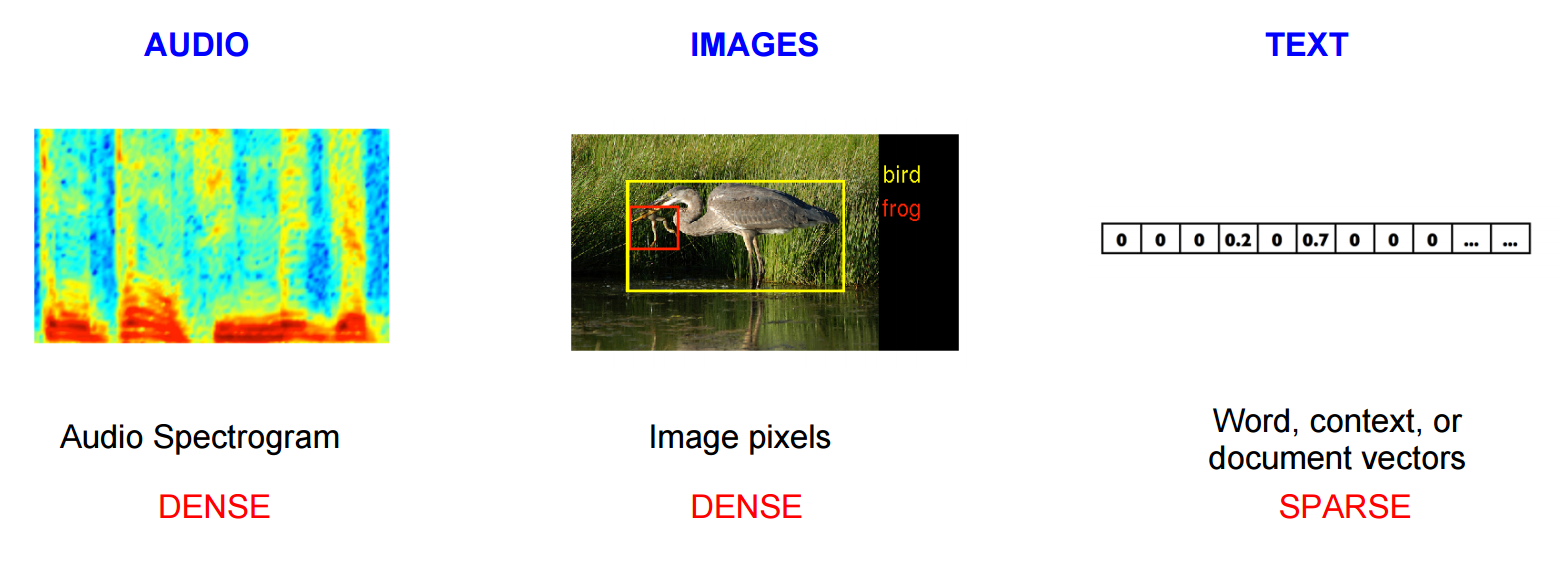
\includegraphics[width=.7\linewidth]{../article/img/audio-image-text}\\
  {[}TensorFlow 2016{]}
\end{center}
\vfill
\begin{itemize}
\item Natural language processing systems can treat words as atomic symbols, encoded as indexes.
\item E.g.\ 'apple' might become index \textit{Id123} and 'orange' becomes index \textit{Id124}
\item This way of encoding is very sparse, and arbitrary.
\item No representation of the relationship between these word types (such as both are fruit, \dots).
\end{itemize}
\vfill

%%%%%%%%%%%%%%%%%%%%%%%%%%%%%%%%%%%%%%%%%%%%%%%%%%%%%%%%%%%%%%%%%%%%%%%%%%%%%%%%
\NewPage\headline{Word Embeddings} 
\hypertarget{sli:word-embeddings}{}

\begin{minipage}[b]{.4\linewidth}
  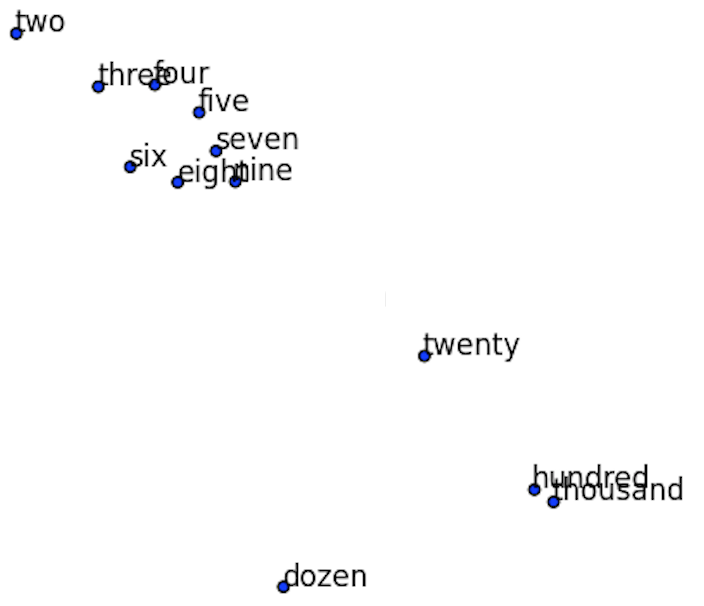
\includegraphics[width=\linewidth]{../article/img/word-embeddings-numbers}\\
  Embeddings visualized {[}Peirsman 2015{]}
\end{minipage}
\begin{minipage}[b]{.6\linewidth}
\begin{itemize}
\item A statistical model should be able to learn relationships between word types.
\item Transform a word type $w$ and turn it into an embedding $e_w = v(w) \in \mathbb{R}^d$
\item Words with a similar meaning should be mapped to (geometrically) nearby points in the vector space.
\item The dimension $d$ should be low compared to the vocabulary size.
\item Capture the intuition that words may be similar along different dimensions.
\end{itemize}
\end{minipage}

%%%%%%%%%%%%%%%%%%%%%%%%%%%%%%%%%%%%%%%%%%%%%%%%%%%%%%%%%%%%%%%%%%%%%%%%%%%%%%%%
\NewPage\headline{Word Embeddings} 
\hypertarget{sli:goals}{}

\vfill
 To this end there are some assumptions we make:
\begin{itemize}
\item Words which share semantic meaning tend to occur in the same contexts (Distributional Hypothesis)
\item The composition of words themselves can sometimes hint at similarities (e.g.\ 'apple' \textit{vs} 'apples')
\end{itemize}
\vfill



%%%%%%%%%%%%%%%%%%%%%%%%%%%%%%%%%%%%%%%%%%%%%%%%%%%%%%%%%%%%%%%%%%%%%%%%%%%%%%%%
\NewPage\headline{General Approach for Word Embeddings} 

\vfill
Generating word embeddings within a NNLM to better estimate $p(w_i | w_1,\dots,w_{i-1})$
\begin{enumerate}
\item Associate each word $w$ in the vocabulary $V$ with a word embedding $e_w$
\item Express the joint probability function for the word sequence $w_1,\dots,w_{i-1}$ in terms of these embeddings.
\item Simultaniously learn the word embeddings and the parameters of the probability function.
\end{enumerate}
\vfill


%%%%%%%%%%%%%%%%%%%%%%%%%%%%%%%%%%%%%%%%%%%%%%%%%%%%%%%%%%%%%%%%%%%%%%%%%%%%%%%%
\NewPage\headline{Continuous Space Language Model}
\hypertarget{sli:simple}{}

\vfill
\begin{minipage}[c]{.5\linewidth}
    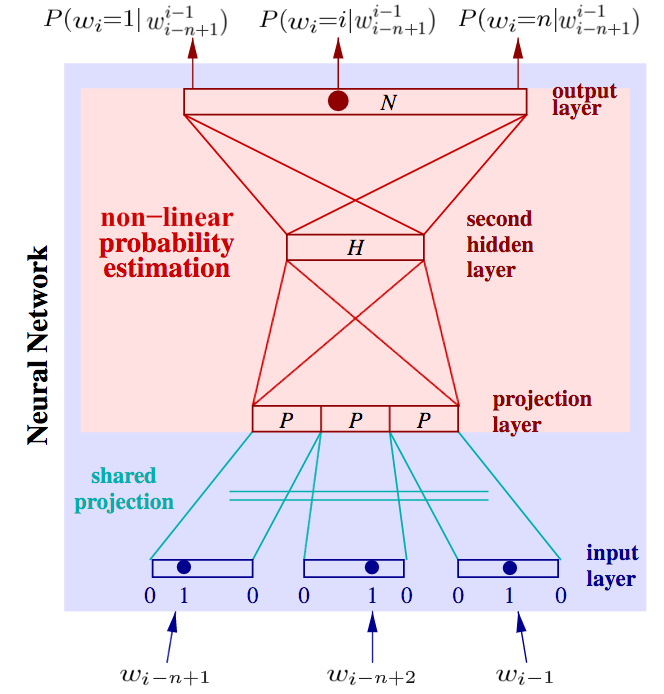
\includegraphics[width=\linewidth]{../article/img/classic_nnlm}\\
    {[}Schwenk 2007{]}
\end{minipage}
\begin{minipage}[c]{.5\linewidth}
\begin{itemize}
\item The context for $w_i$ is approximated with n-grams.
\item Input word types are encoded as one-hot vectors.
\item First Hidden Layer: Lookup table $P \in \mathbb{R}^{d \times |V|}$, projects the input into a continouus vector space.
\item The word embedding $e_w$ is the output of layer $P$.
\item Second Hidden Layer: Estimates the joint probability of the word sequence
\item The Softmax-Layer projects this up to vocabulary size $|V|$
    %, calculating $p(w_i = k | w_1,\dots,w_{i-1})$ for every word-type $k \in V$.
\end{itemize}
\end{minipage}
\vfill

%%%%%%%%%%%%%%%%%%%%%%%%%%%%%%%%%%%%%%%%%%%%%%%%%%%%%%%%%%%%%%%%%%%%%%%%%%%%%%%%
\NewPage\headline{Resulting Embeddings}

\begin{center}
  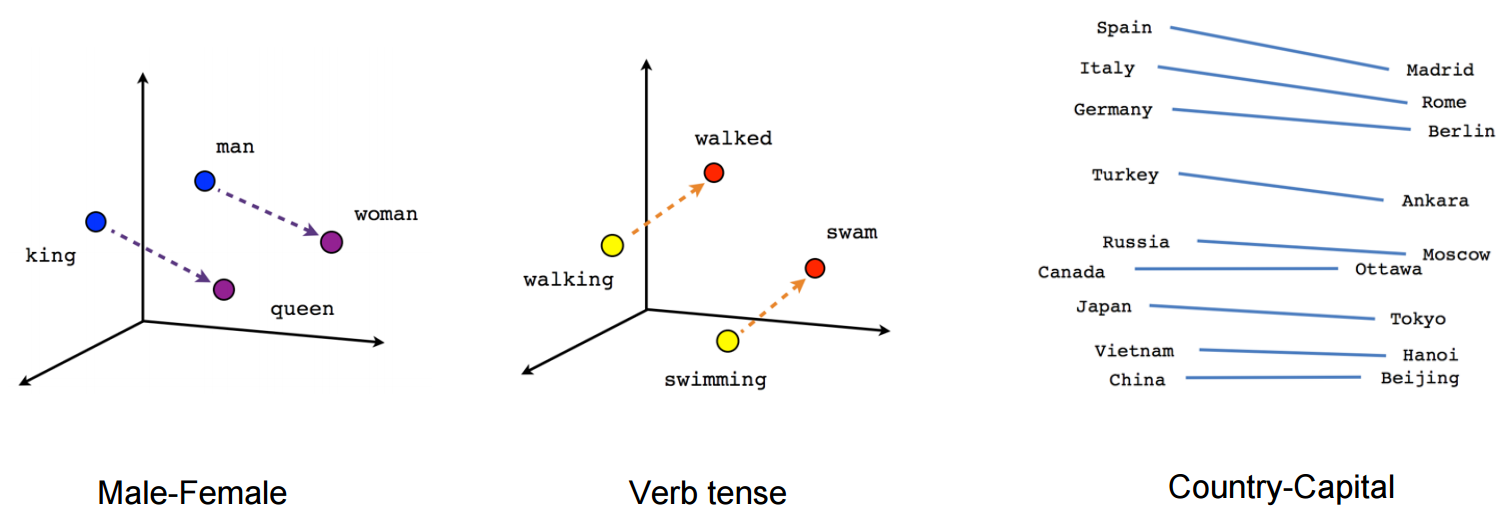
\includegraphics[width=.8\textwidth]{../article/img/linear-relationships}\\
  {[}TensorFlow 2016{]}
\end{center}

\vfill
\begin{itemize}
\item This setup can be used to generate a large table of word embeddings.
\item Lookup table can be reused for other tasks (if there is not enough training data).
\item E.g.\ [Mikolov et al 2013] have created a model which can encode complex patterns:
\item ${\displaystyle v(\mathrm {king} )-v(\mathrm {male} )+v(\mathrm {female} )\approx v(\mathrm {queen} )}$.
\end{itemize}
\vfill



%%%%%%%%%%%%%%%%%%%%%%%%%%%%%%%%%%%%%%%%%%%%%%%%%%%%%%%%%%%%%%%%%%%%%%%%%%%%%%%%
%\NewPage\headline{Reminder: Softmax-Layer}
%
%\vfill
%\begin{minipage}[b]{.4\linewidth}
%  \begin{center}
%    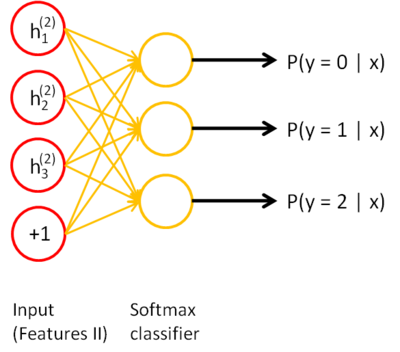
\includegraphics[width=\linewidth]{../article/img/softmax_layer}\\
%    $p_k = \sigma(\mathbf{z})_k = \frac{e^{z_k}}{\sum_{k=1}^{|V|} e^{z_k}}$
%  \end{center}
%\end{minipage}
%\begin{minipage}[b]{.6\linewidth}
%  \begin{itemize}
%  \item The input vector $z$ is computed over the vocabulary: $z_k \forall k \in V$.
%  \item The result of the outputs can be interpreted as posterior probabilities.
%  \item Probability given the context: $p_k = p(w_i = k | w_{i-n+1}^{i-1})$
%  \end{itemize}
%\end{minipage}
% \vfill


%%%%%%%%%%%%%%%%%%%%%%%%%%%%%%%%%%%%%%%%%%%%%%%%%%%%%%%%%%%%%%%%%%%%%%%%%%%%%%%%
\NewPage\headline{Shortcomings}

\vfill
\begin{itemize}
\item A model with a lookup table treats each word embedding as independent from each other. 
\begin{itemize}
  \item The model captures smililar linear correspondences between words embeddings.
  \item E.g.\ \textit{cat} and \textit{apple} compared to \textit{cats} and \textit{apples}.
  \item It doesn't capture that the added \textit{s} is responsible for this transformation.
  \item The model doesn't examine lexical similarities between words.
  \item It doesn't capture morphological word transformations: e.g.\ \textit{test} vs.\ \textit{testing}
\end{itemize}
\item A word lookup table cannot easily deal with unknown words.
\item The lookup table contains at least $|V| \times d$ parameters. This can require large amount of memory for tasks with large vocabularies.
\end{itemize}
\vfill

%%%%%%%%%%%%%%%%%%%%%%%%%%%%%%%%%%%%%%%%%%%%%%%%%%%%%%%%%%%%%%%%%%%%%%%%%%%%%%%%

\NewPage\headline{Possible Solutions}

\vfill
Some requirements should be satisfied by a better model:
\begin{itemize}
  \item The model should capture\textsuperscript{*} orthographic similarities between words
        e.g.\ \textit{test} vs.\ \textit{testing} (Compositional effects).
  \item The model must still capture functionally similar words, with no orthographic
        similarities e.g.\ \textit{rich} vs.\ \textit{affluent}.
  \item However not all similary spelled words have similar meanings e.g.\ \textit{butter} vs.\ \textit{batter}.
  \item The resulting model should be able to replace the previous projection layer.
  \item Idea: Break down words into smaller atomic units and try to \textit{compose} them into word embeddings.
\end{itemize}
\vfill
{\footnotesize *) In terms of geometric locality}


%%%%%%%%%%%%%%%%%%%%%%%%%%%%%%%%%%%%%%%%%%%%%%%%%%%%%%%%%%%%%%%%%%%%%%%%%%%%%%%%
\NewPage\headline{Possible Solution 1: Morpheme-based Embeddings}

\vfill
\begin{itemize}
\item Morphemes are the smallest defined grammatical unit of a language.
\item E.g.\ "Unbreakable" comprises three morphemes: 
  \begin{enumerate}
    \item un-
    \item -break-
    \item -able
  \end{enumerate}
\item Use morphemes as input and compose them into the word embeddings.
\item Requires a morphological analyser: Extra processing step.
\item Each target language requires an extra morpological analyser.
\item The quality of the model depends on the analyser.
\end{itemize}
\vfill

%%%%%%%%%%%%%%%%%%%%%%%%%%%%%%%%%%%%%%%%%%%%%%%%%%%%%%%%%%%%%%%%%%%%%%%%%%%%%%%%
\NewPage\headline{Possible Solution 2: Character-based Embeddings}

\vfill
\begin{itemize}
  \item Break down words into characters
  \item Represent characters as real valued feature vectors (character embeddings).
  \item Feed them to an recurrent neural net, which "remembers" each character.
  \item Learn character embeddings simultaniously with other model parameters.
\end{itemize}
\vfill




%%%%%%%%%%%%%%%%%%%%%%%%%%%%%%%%%%%%%%%%%%%%%%%%%%%%%%%%%%%%%%%%%%%%%%%%%%%%%%%%
%\NewPage\headline{Repetition: Long-Short Term Memory}
%
%\vfill
%\begin{figure}[H]
%\begin{center}
%  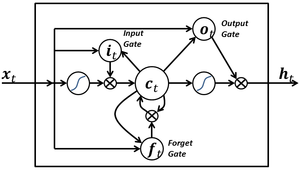
\includegraphics[width=.5\textwidth]{../article/img/Long_Short_Term_Memory}
%\end{center}
%\end{figure}
%\vfill
%Given the input vectors $x_1,\dots,x_m$ a LSTM computes the sequence $h_1,\dots, h_{m+1}$
%\begin{equation}
%\begin{aligned}  
%  i_t &=\sigma(W_{ix} * x_t  + W_{ih} * h_{t-1} + W_{ic} * c_{t-1} + b_i) \\  
%  f_t &=\sigma(W_{fx} * x_t  + W_{fh} * h_{t-1} + W_{fc} * c_{t-1} + b_f) \\
%  o_t &=\sigma(W_{ox} * x_t  + W_{oh} * h_{t-1} + W_{oc} * c_t + b_o) \\  
%  c_t &= f_t \odot c_{t-1} + i_t \odot \tanh(W_{cx} * x_t  + W_{ch} * h_{t-1} + b_c) \\ 
%  h_t &= o_t \odot \tanh(c_t) 
% \end{aligned}
% \end{equation}
% \vfill
% LSTM's avoid the vanishing gradient problem, because
% the activation function in $c_t$ is the identity function.
% \vfill

%%%%%%%%%%%%%%%%%%%%%%%%%%%%%%%%%%%%%%%%%%%%%%%%%%%%%%%%%%%%%%%%%%%%%%%%%%%%%%%%
\NewPage\headline{Character-based Word-Embeddings}

\vfill
The "Compositional Character to Word" (C2W) model:
\begin{enumerate}
\item A word $w$ with length $m$ is decomposed into characters $c_1, \dots, c_m$ from the alphabet $C$.
\item Transform characters into a sequence of character embeddings $e_{c_1}, \dots, e_{c_m}$.
\item The sequence is "read" one-by-one \textbf{forwards} as well as \textbf{backwards} by two LSTMs.
\item During "reading" the sequence is composed into the forward state $s_m^f$ and backward state $s_1^b$.
\item The two states are recomposed to form the word-embedding $e_w$.
\end{enumerate}
\vfill

%%%%%%%%%%%%%%%%%%%%%%%%%%%%%%%%%%%%%%%%%%%%%%%%%%%%%%%%%%%%%%%%%%%%%%%%%%%%%%%%
\NewPage\headline{Compositional Character to Word Model}

\begin{minipage}[c]{.5\linewidth}
  \begin{center}
    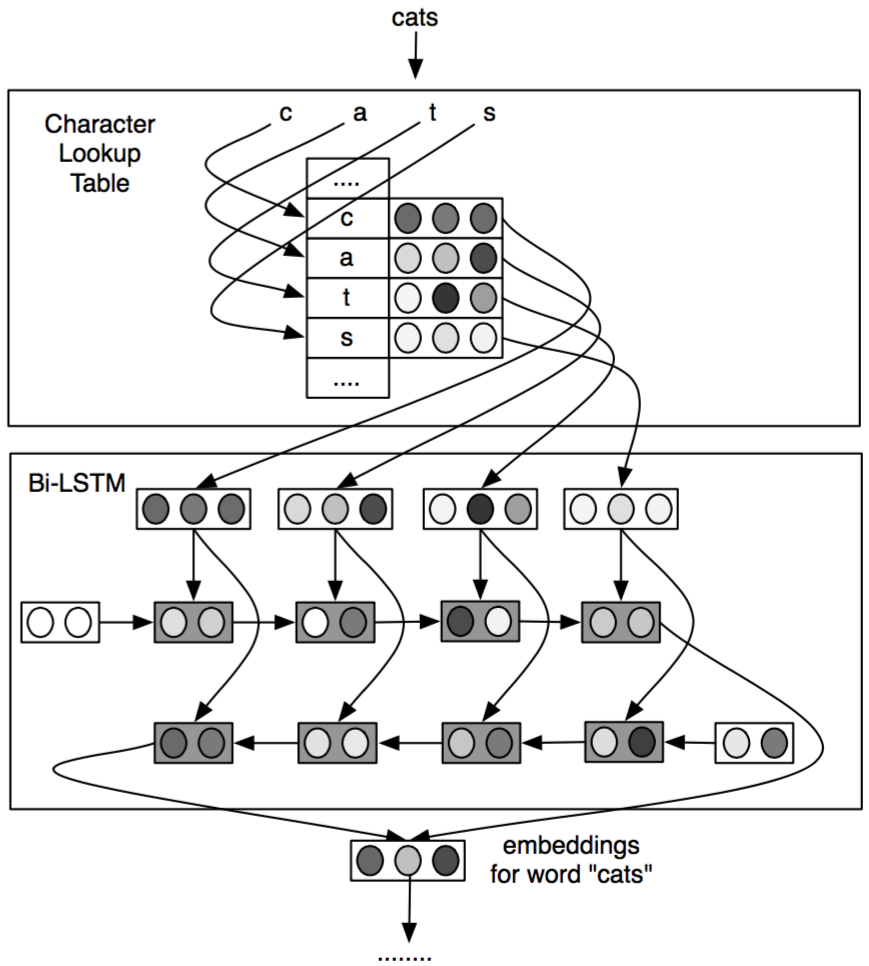
\includegraphics[width=\linewidth]{../article/img/bi-lstm-emeddings}\\
    {[}Wang Ling et al 2015{]}
  \end{center}
\end{minipage}
\begin{minipage}[c]{.5\linewidth}
The C2W model is visualized for input "cats":
  \begin{itemize}
  \item Squared boxes represent vectors of neuron activations.
  \item Shaded boxes indicate a nonlinear output.
  \item The two actual LSTM units are displayed unfolded.
  \end{itemize}
\end{minipage}

%%%%%%%%%%%%%%%%%%%%%%%%%%%%%%%%%%%%%%%%%%%%%%%%%%%%%%%%%%%%%%%%%%%%%%%%%%%%%%%%
\NewPage\headline{C2W-Model: Layers}

\begin{minipage}[c]{.5\linewidth}
  \begin{center}
    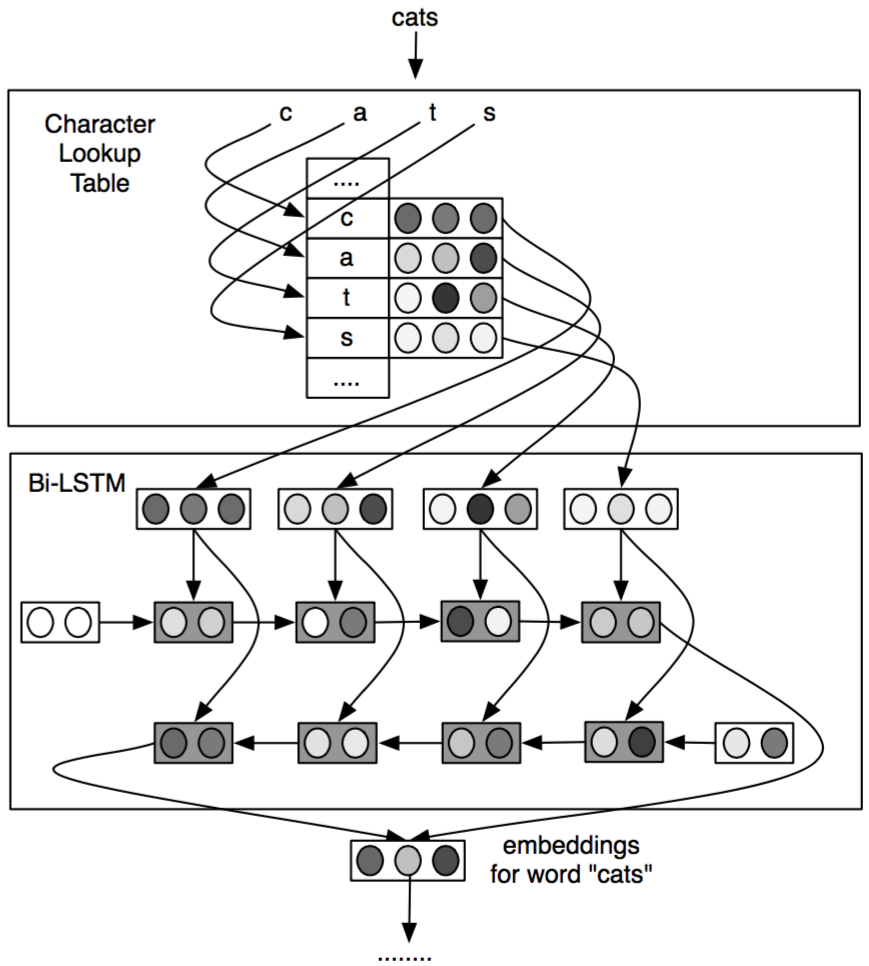
\includegraphics[width=\linewidth]{../article/img/bi-lstm-emeddings}\\
    {[}Wang Ling et al 2015{]}
  \end{center}
\end{minipage}
\begin{minipage}[c]{.5\linewidth}
  \begin{enumerate}
  \item Table of character embeddings.
  \item Bidirectional-LSTM layer, processing forward- and backward-sequences of character embeddings.
  \item The combining layer, to merge the two outputs from the Bi-LSTM.
  \end{enumerate}
\end{minipage}


%%%%%%%%%%%%%%%%%%%%%%%%%%%%%%%%%%%%%%%%%%%%%%%%%%%%%%%%%%%%%%%%%%%%%%%%%%%%%%%%
\NewPage\headline{C2W-Model: Character-Lookup Table}

\begin{figure}[H]
\begin{center}
  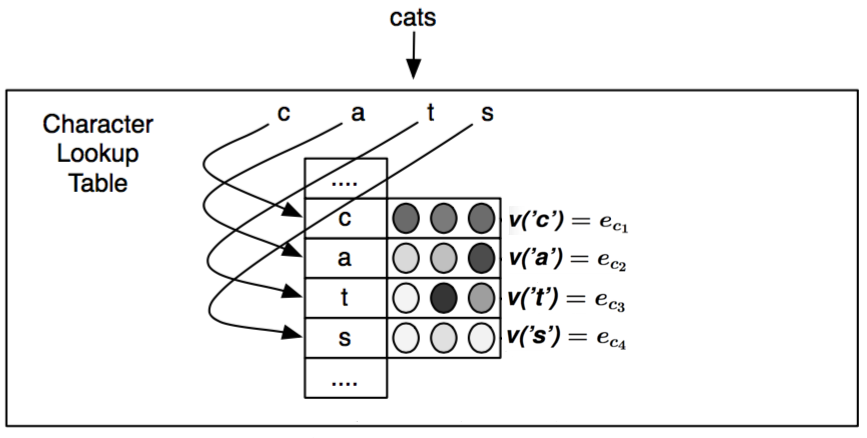
\includegraphics[width=.5\textwidth]{../article/img/character-lookup}
\end{center}
\end{figure}

\vfill
\begin{itemize}
  \item Table of $d_C$ parameters $P_C \in \mathbb{R}^{d_C \times |C|}$ .
  \item Each Input character $c$ is transformed into a $d_C$-dimensional feature vector $e_{c}$.
  % \item We define the projection of characters as $e_{c_j}^C = P_C * 1_{c_j}$.

  \item The dimension $d_C$ becomes a hyperparameter of the model.
  \item Basically similar to the previous projection layer for words.
\end{itemize}
\vfill



%%%%%%%%%%%%%%%%%%%%%%%%%%%%%%%%%%%%%%%%%%%%%%%%%%%%%%%%%%%%%%%%%%%%%%%%%%%%%%%%
\NewPage\headline{Reminder: Long Short-Term Memory}


\begin{minipage}[c]{.5\linewidth}
  \begin{center}
   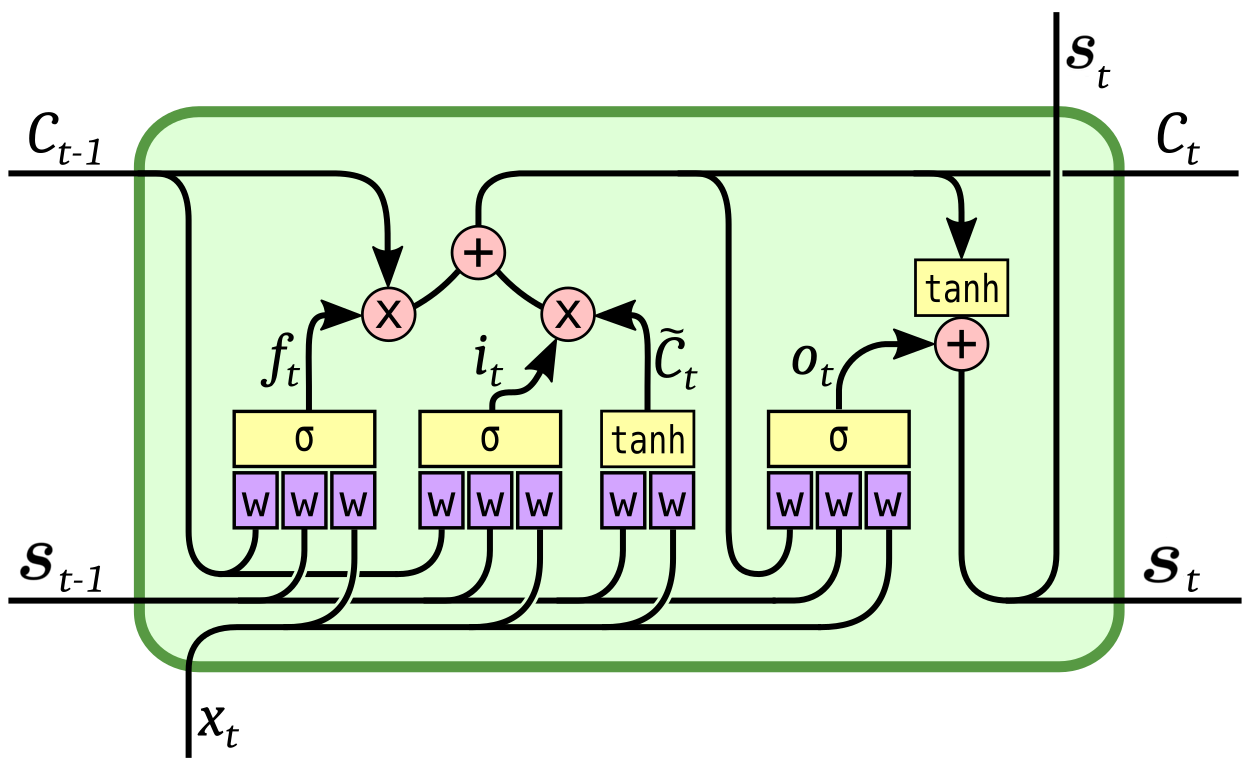
\includegraphics[width=\textwidth]{lstm-peepholes}
  \end{center}
\end{minipage}
\begin{minipage}[c]{.5\linewidth}
  \begin{itemize}
\item Designed to "remember" inputs over arbitary distances and "forget" them when necessary
\item Gate \(i_t\) to determine when to learn an input value
\item Gate \(f_t\) to determine if it should continue to remember or forget the currently stored value
\item Gate \(o_t\) to determine wether it should output the value.
\item Additionally and bias values not explicitly displayed here.
\item The dimension $d_{CS}$ of the LSTM state becomes another hyperparameter.
\end{itemize}
\end{minipage}




%%%%%%%%%%%%%%%%%%%%%%%%%%%%%%%%%%%%%%%%%%%%%%%%%%%%%%%%%%%%%%%%%%%%%%%%%%%%%%%%
\NewPage\headline{C2W-Model: Bidirectional LSTM Layer}

\vfill
\begin{figure}[H]
\begin{center}
  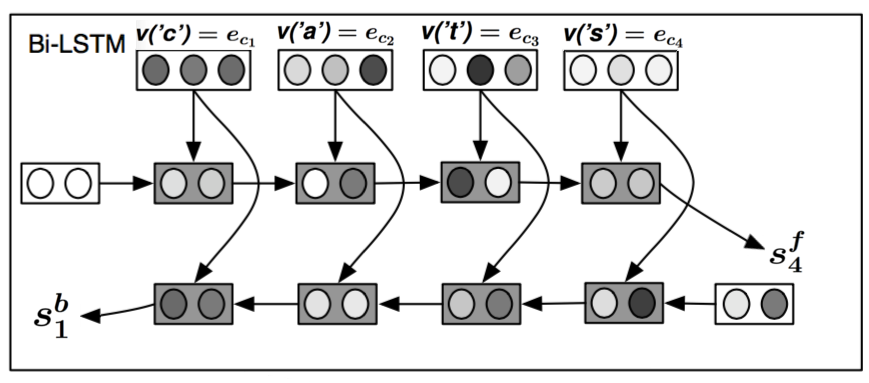
\includegraphics[width=.5\linewidth]{../article/img/brnn-unfolded}
\end{center}
\end{figure}
\begin{itemize}
\item Present the character sequence forwards and backwards to two separate LSTMs.
\item Yields the forward state sequence $s_{1}^f, \dots, s_{m}^f$ and backward state sequence $s_{m}^b, \dots, s_{1}^b$.
\item The network has simultanious access to all inputs before and after the current one.
\item No need for fixed window sizes for the input, the net decides how much context to use.
\end{itemize}
\vfill


%%%%%%%%%%%%%%%%%%%%%%%%%%%%%%%%%%%%%%%%%%%%%%%%%%%%%%%%%%%%%%%%%%%%%%%%%%%%%%%%
\NewPage\headline{C2W-Model: Combining Layer}

\vfill
\begin{itemize}
\item Combines the last forward state $s_{m}^f$ and the last backward state $s_{1}^b$
\item $e_{w} = D^f s_{m}^f + D^b s_{0}^b + b_d$
\item The variables $D^f, D^b, b_d$ are the weights which determine how the states are combined.
\item Automatically learns to determine how much each context is used.
\end{itemize}
\vfill


%%%%%%%%%%%%%%%%%%%%%%%%%%%%%%%%%%%%%%%%%%%%%%%%%%%%%%%%%%%%%%%%%%%%%%%%%%%%%%%%
\NewPage\headline{C2W-Model vs Lookup Tables}

\begin{minipage}[b]{.5\linewidth}
    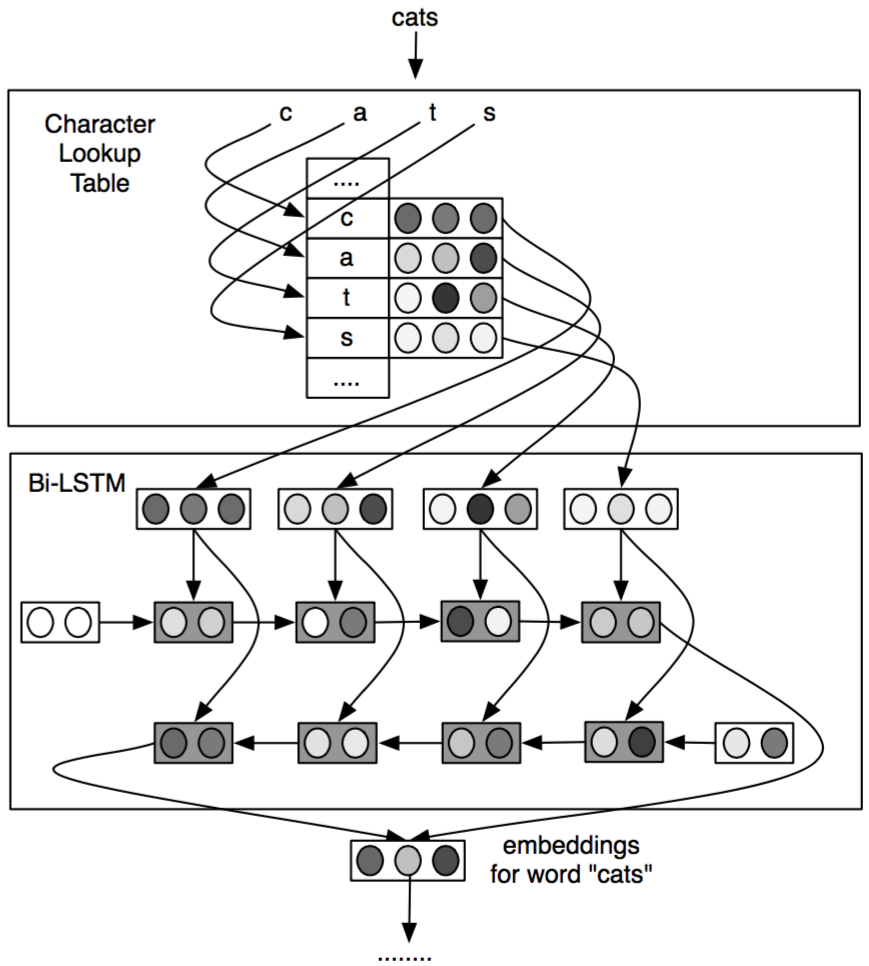
\includegraphics[width=\linewidth]{../article/img/bi-lstm-emeddings}\\
\end{minipage}
\begin{minipage}[b]{.5\linewidth}
    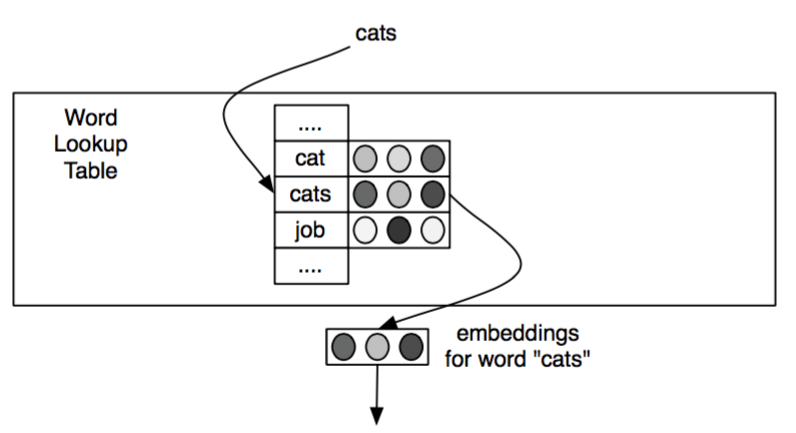
\includegraphics[width=\linewidth]{../article/img/word-lookup}
\end{minipage}
\vfill

%%%%%%%%%%%%%%%%%%%%%%%%%%%%%%%%%%%%%%%%%%%%%%%%%%%%%%%%%%%%%%%%%%%%%%%%%%%%%%%%
\NewPage\headline{C2W-Model vs Word Lookup Tables}

\begin{itemize}
\item Lookup Tables are conceptually much simpler, but requires a lot of parameters ($|V| \times d$).
\item The C2W model uses less parameters (more in the evaluation section).
\item The C2W model can easily be used for open vocabulary tasks.
\item Looking up a word embedding is in $O(1)$, whereas the C2W model has to compute the embedding
  \begin{itemize}
  \item Can be aliviated by caching $e_w$ for frequently occuring words.
  \item However cached values still need to be recomputed when parameters change during training time.
  \end{itemize}
\end{itemize}
\vfill



%%%%%%%%%%%%%%%%%%%%%%%%%%%%%%%%%%%%%%%%%%%%%%%%%%%%%%%%%%%%%%%%%%%%%%%%%%%%%%%%
\NewPage\headline{Experimentation}

\vfill
We are going to introduce three use cases, where a C2W based model either:
\begin{itemize}
\item Outperforms a model which uses much more parameters.
\item Yields comparable results without relying on manually engineered features.
\end{itemize}
\vfill
\begin{description}
\item [Wang Ling et al 2015 :] Language Modelling 
\item [Wang Ling et al 2015 :] Part-Of-Speech Tagging
\item [Faruqui et al 2015 :] Morphological Inflection Generation
\end{description}
\vfill


%%%%%%%%%%%%%%%%%%%%%%%%%%%%%%%%%%%%%%%%%%%%%%%%%%%%%%%%%%%%%%%%%%%%%%%%%%%%%%%%
\NewPage\headline{Application 1: Language Modeling}

\begin{center}
    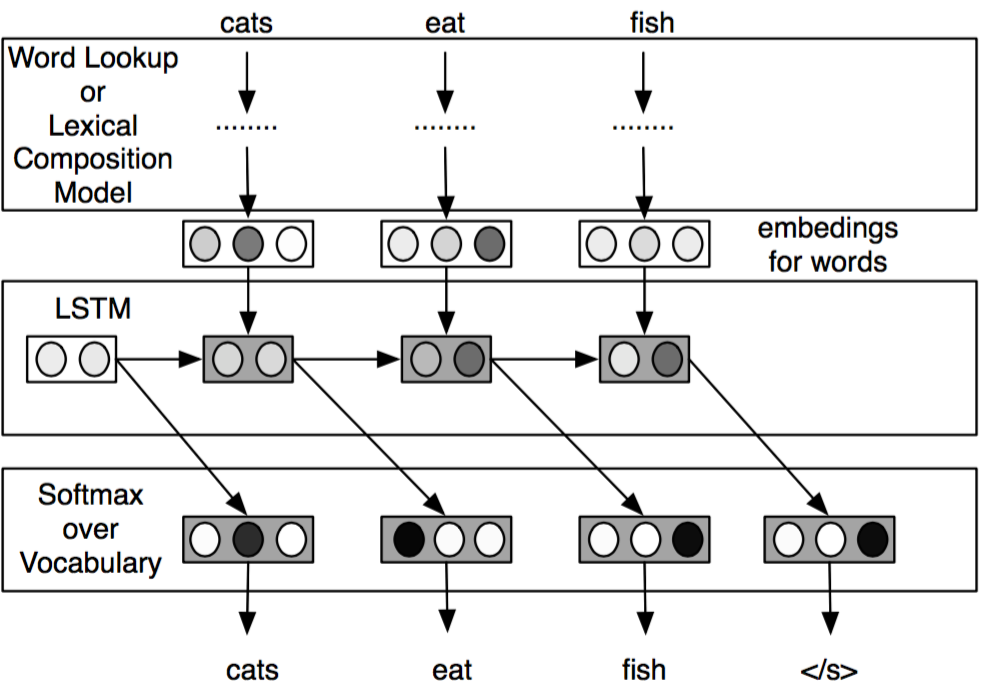
\includegraphics[width=.5\linewidth]{../article/img/c2w-language-model}
\end{center}
\vfill
\begin{itemize}
\item Computes the joint probability for the word sequence $w_1,\dots,w_{i-1}$ with a hidden LSTM layer.
\item Test two versions of this NLM: One with the C2W model and one with a word lookup table as projection layer. 
\item Compare accuracy of these two versions.
\end{itemize}
\vfill


%%%%%%%%%%%%%%%%%%%%%%%%%%%%%%%%%%%%%%%%%%%%%%%%%%%%%%%%%%%%%%%%%%%%%%%%%%%%%%%%
\NewPage\headline{Application 1: Training \& Testing Data}

\vfill
\begin{itemize}
\item Perform testing on English, Portuguese, Catalan, German and Turkish.
\item Choosen because these are morphologically rich languages.
\item Training data was obtained by randomly extracting wikipedia articles until 1 million words were obtained.
\item Additionaly $20000$ words were obtained for testing.
\end{itemize}
\vfill


%%%%%%%%%%%%%%%%%%%%%%%%%%%%%%%%%%%%%%%%%%%%%%%%%%%%%%%%%%%%%%%%%%%%%%%%%%%%%%%%
\NewPage\headline{Application 1: Parameter Count}

\vfill
\begin{itemize}
\item The word embedding dimension is set to $d = 50$.
  \begin{itemize}
  \item A word lookup table contains at least $d \times |V|$ parameters, 
  \item A language with $80000$ words will have at least 4 million parameters. 
  \end{itemize}
\item The C2W model has two additional hyperparameters which are set to $d_C = 50$ and $d_{CS} = 150$
\begin{itemize}
  \item The LSTMs use 8 matrices of size $d_{CS} \times d_C + 2 d_{CS}$ (one for each decision gate).
  \item The $d \times 2d_{CS}$ parameters in the combining output layer.
  \item The $d_C \times |C|$ parameters in the character table.
  \item For english this works out to roughly $180000$ parameters.
\end{itemize}
\end{itemize}
\vfill

%%%%%%%%%%%%%%%%%%%%%%%%%%%%%%%%%%%%%%%%%%%%%%%%%%%%%%%%%%%%%%%%%%%%%%%%%%%%%%%%
\NewPage\headline{Reminder: Perplexity}

\vfill
\begin{itemize}
\item Measure of how well a probability distribution predicts sample data.
\item Can be interpreted as the number of choices per word position.
\item Defined as $2^{H(p)}=2^{-\sum_x p(x)\log_2 p(x)}$
\item To minimize the perplexity value means to have a better fitting language model.
\end{itemize}
\vfill

%%%%%%%%%%%%%%%%%%%%%%%%%%%%%%%%%%%%%%%%%%%%%%%%%%%%%%%%%%%%%%%%%%%%%%%%%%%%%%%%
\NewPage\headline{Application 1: Evaluation}

\begin{table}
\centering
\begin{tabular}{ l | l l l l l }
  %           & \multicolumn{3}{c|}{Fusional} &   \multicolumn{2}{|c|}{Agglutinative} \\ \hline
  Perplexity   & English & Portugese & Catalan & German & Turkish \\
  %5-gram KN    & 70.72   & 58.73     &   39.83 & 59.07  & 52.87   \\
  Word Lookup  & 59.38   & 46.17     &   35.34 & 43.02  & 44.01   \\
  C2W Model    & \textbf{57.39}   & \textbf{40.92}     &   \textbf{34.92} & \textbf{41.94}  & \textbf{32.88}   \\
  \#Parameters  &         &           &         &        &         \\
  Word Lookup  & 4.3M    & 4.2M      &  4.3M   & 6.3M   & 5.7M   \\
  C2W Model    & \textbf{180K}    & \textbf{178K}      &  \textbf{182K}   & \textbf{183K}   & \textbf{174K}   \\

\end{tabular}
\caption{Perplexities and test configuration~{[}Wang Ling et al 2015{]}.}
\end{table}
\vfill
\begin{itemize}
\item Training is performed with mini-batch gradient descent with 100 sentences each.  
\item Speed of both model versions is aproximatly 300 words per second, main bottleneck is the softmax layer.
\item In general C2W outperforms word lookup tables and requires less parameters.
\end{itemize}
\vfill

%%%%%%%%%%%%%%%%%%%%%%%%%%%%%%%%%%%%%%%%%%%%%%%%%%%%%%%%%%%%%%%%%%%%%%%%%%%%%%%%
\NewPage\headline{Application 1: Nonce Words}

\begin{table}
\centering
\begin{tabular}{ c | c }
   Noahshire &  phding \\ \hline
   Nottinghamshire & mixing \\
   Bucharest & modelling \\
   Saxony & styling \\
   Johannesburg & blaming \\
   Gloucestershire & christening \\
\end{tabular}
\caption{Nonce words and their most similar words from the vocabulary~{[}Wang Ling et al 2015{]}.}
\end{table}

\vfill
\begin{itemize}
\item Nonce words are words created for use in a single occasion.
\item The C2W model is able to generate embeddings for these words.
\item No need for an OOV token for out of vocabulary words.
\end{itemize}
\vfill

%%%%%%%%%%%%%%%%%%%%%%%%%%%%%%%%%%%%%%%%%%%%%%%%%%%%%%%%%%%%%%%%%%%%%%%%%%%%%%%%
\NewPage\headline{Application 2: Part-Of-Speech Tagging}

\vfill
\begin{itemize}
\item Process of labeling words as corresponding to a particular part of speech
\item For example a simple tagging would be to identify words as nouns, verbs, adjectives, adverbs, etc.
\item One use of this is to disambiguate homonyms:\\ For Example "I fish a fish" should become "Je pêche un poisson" in french.
\item By tagging the first occurance of "fish" as verb and the second as noun, they are now distinct.
\end{itemize}
\vfill

%%%%%%%%%%%%%%%%%%%%%%%%%%%%%%%%%%%%%%%%%%%%%%%%%%%%%%%%%%%%%%%%%%%%%%%%%%%%%%%%
\NewPage\headline{Application 2: Part-Of-Speech Tagging}

\begin{center}
    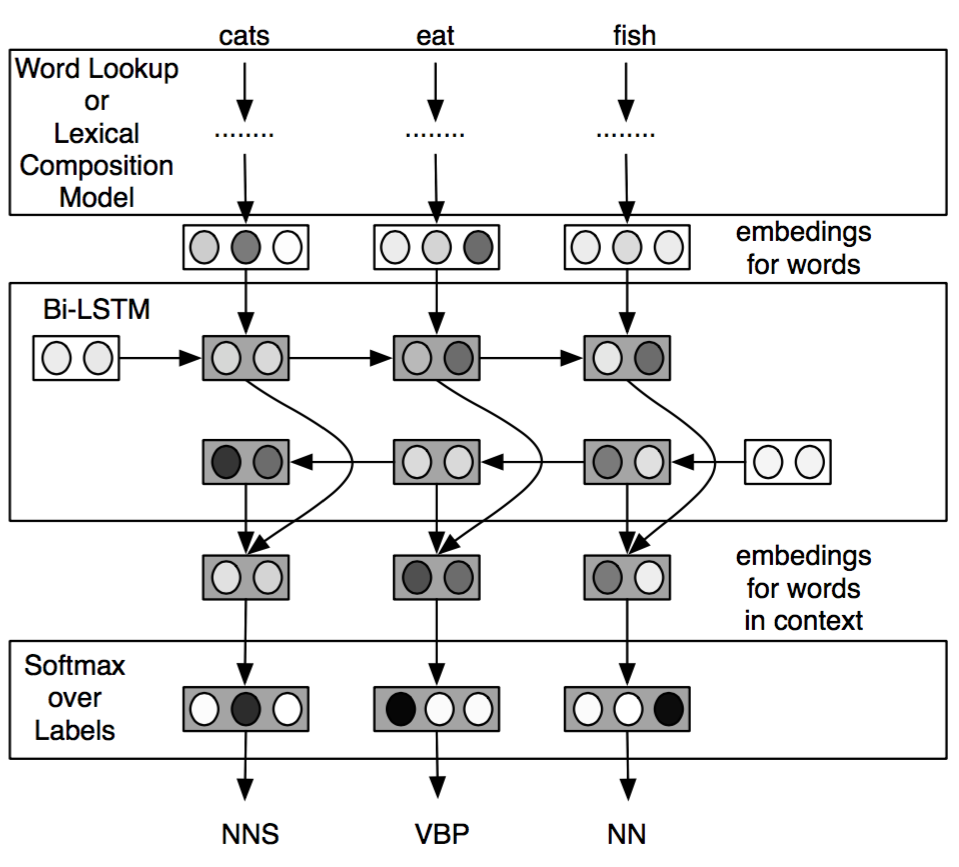
\includegraphics[width=.5\linewidth]{../article/img/part-of-speech}
\end{center}
\vfill
\begin{itemize}
\item Conceptually similar to the previous NLM model.
\item We don't just use a single LSTM block, but a bidirectional LSTM.
\item The softmax layer computes over all possible labels instead of the vocabulary
\end{itemize}
\vfill

%%%%%%%%%%%%%%%%%%%%%%%%%%%%%%%%%%%%%%%%%%%%%%%%%%%%%%%%%%%%%%%%%%%%%%%%%%%%%%%%
\NewPage\headline{Application 2: Testing Setup}

\vfill
\begin{itemize}
\item For english annotated sentences of the Wall Street Journal from the "Penn Treebank" dataset are used.
\item For other languages data provided by the "Conference on Natural Language Learning" was used.
\item The dimension of the states in the additional Bi-LSTM layer are set to 50.
\item Out of vocabulary words are replaced with an OOV token.
\end{itemize}
\vfill

%%%%%%%%%%%%%%%%%%%%%%%%%%%%%%%%%%%%%%%%%%%%%%%%%%%%%%%%%%%%%%%%%%%%%%%%%%%%%%%%
\NewPage\headline{Application 2: Evaluation}

\begin{center}
    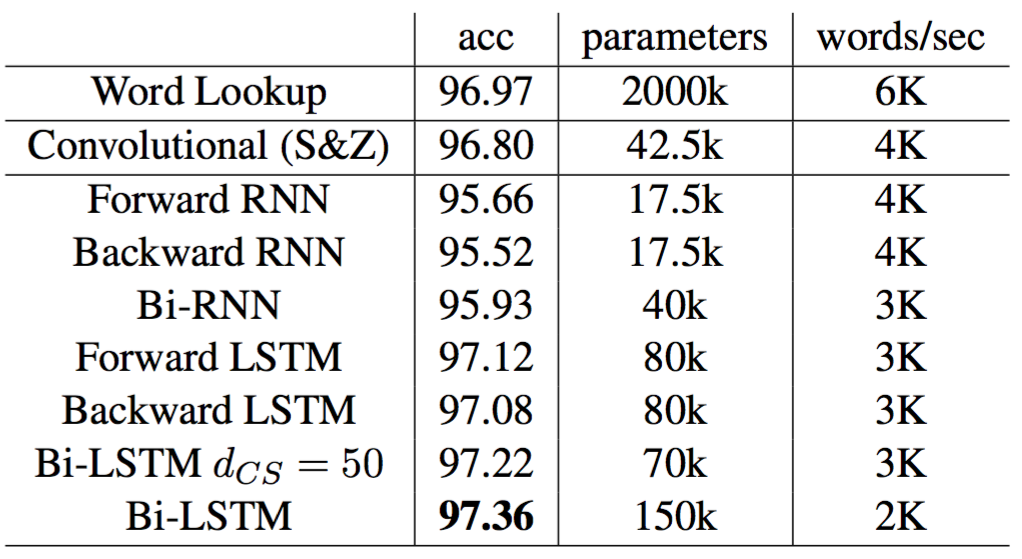
\includegraphics[width=.5\linewidth]{evaluation_pos_2}\\
\end{center}

\vfill
\begin{itemize}
\item As previously the C2W based POS-model is compared with versions using different
      word representation models.
\item Table contains accuracies for the english WSJ dataset only.
  \begin{itemize}
  \item There are different configurations using regular RNNs and LSTMs.
  \item The LSTMs always outperforms regular RNNs by about 2\%.
  \item Row "Convolutional (S\&Z)" contains results of a convolutional model from [Santos and Zadrozny, 2014].
  \end{itemize}
\end{itemize}
\vfill
{\footnotesize [Santos and Zadrozny, 2014]: Learning Character-level Representations for Part-of-Speech Tagging}


%%%%%%%%%%%%%%%%%%%%%%%%%%%%%%%%%%%%%%%%%%%%%%%%%%%%%%%%%%%%%%%%%%%%%%%%%%%%%%%%
\NewPage\headline{Application 2: Evaluation}

\begin{center}
      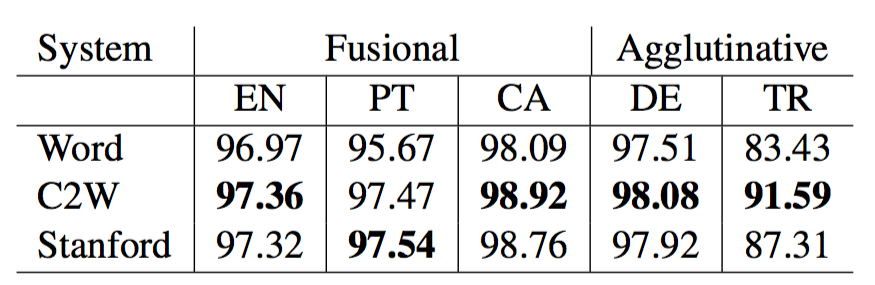
\includegraphics[width=.5\linewidth]{evaluation_pos}
\end{center}

\vfill
\begin{itemize}

\item This table contains testing results for a number of languages.
\item As previously the row "word" contains results for a model version using word lookup tables.
\item Additionally it is compared with Stanford’s POS tagger, with the default set of features. 
\end{itemize}
\vfill


%%%%%%%%%%%%%%%%%%%%%%%%%%%%%%%%%%%%%%%%%%%%%%%%%%%%%%%%%%%%%%%%%%%%%%%%%%%%%%%%
\NewPage\headline{Application 3: Morphological Inflection Generation}

\vfill
\begin{table}
\begin{center}
\begin{tabular}{ l l l l }
  \hline
             & singular & plural \\ \hline
  nominative & Kalb & K\"alber \\
  accusative & Kalb & K\"alber \\
  dative & Kalb & K\"albern \\
  genitive & Kalbes & K\"alber \\
\end{tabular}
\end{center}
\caption{Example of an inflection table for the word "Kalb"~[Faruqui et al 2015]}
\end{table}
\vfill
\begin{itemize}
\item We want to perform morphological transformations of words.
\item These kind transformations are very common in languages like turkish or german.
\item Could be used as post- or preprocessing step for machine trainlation.
\end{itemize}
\vfill

%%%%%%%%%%%%%%%%%%%%%%%%%%%%%%%%%%%%%%%%%%%%%%%%%%%%%%%%%%%%%%%%%%%%%%%%%%%%%%%%
\NewPage\headline{Application 3: Overview}

\begin{figure}[H]
\begin{center}
  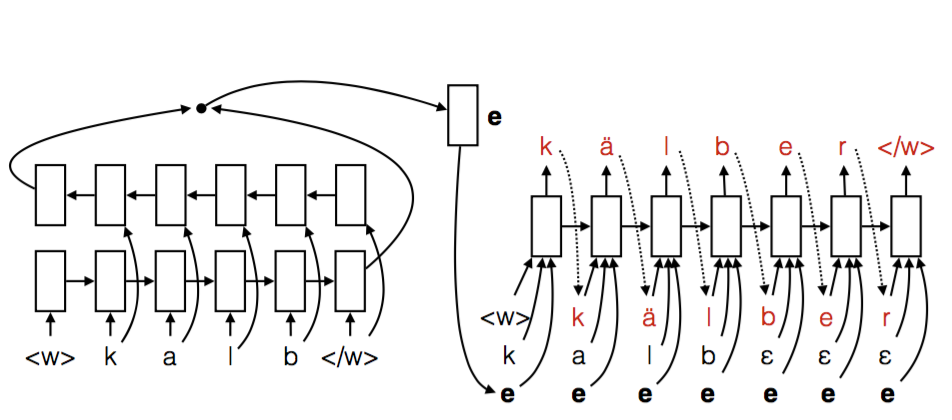
\includegraphics[width=.6\linewidth]{../article/img/inflection-generation}
\end{center}
\end{figure}
\begin{itemize}
\item We use a neuronal encoder - decoder architecture.
\item The word embedding $e$ is used as an intermediate representation.
\item The decoder constructs the inflected version of the word - character by character.
\end{itemize}


%%%%%%%%%%%%%%%%%%%%%%%%%%%%%%%%%%%%%%%%%%%%%%%%%%%%%%%%%%%%%%%%%%%%%%%%%%%%%%%%
\NewPage\headline{Application 3: Overview}

\begin{figure}[H]
\begin{center}
  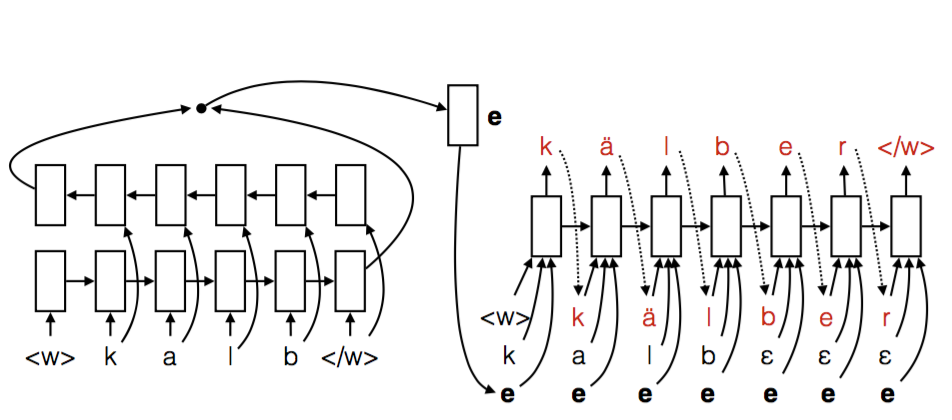
\includegraphics[width=.6\linewidth]{../article/img/inflection-generation}
\end{center}
\end{figure}
\begin{itemize}
\item The encoder part is identically to the C2W model and generates a word embedding $e$.
\item The decoder is just an LSTM unit which receives the following inputs each timestep:
  \begin{enumerate}
    \item The word embedding $e$ from the encoder.
    \item Current character of the original word $c_j$
    \item Previous output of the model
  \end{enumerate}
\end{itemize}


%%%%%%%%%%%%%%%%%%%%%%%%%%%%%%%%%%%%%%%%%%%%%%%%%%%%%%%%%%%%%%%%%%%%%%%%%%%%%%%%
\NewPage\headline{Application 3: Decoder}

\begin{figure}[H]
\begin{center}
  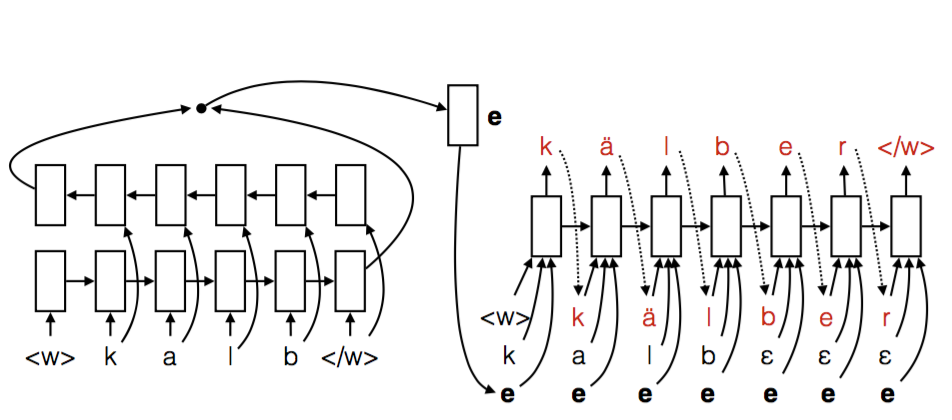
\includegraphics[width=.6\linewidth]{../article/img/inflection-generation}
\end{center}
\end{figure}
\begin{itemize}
\item The decoder output is driven by the characters of the original word
\item There is a chance that output length is greater than the input word length.
\item Once the input word ends, the  $\epsilon$ character is used instead.
\item The decoder stops by outputting the word end token "$<$/w$>$"
\end{itemize}

%%%%%%%%%%%%%%%%%%%%%%%%%%%%%%%%%%%%%%%%%%%%%%%%%%%%%%%%%%%%%%%%%%%%%%%%%%%%%%%%
\NewPage\headline{Application 3: Training \& Testing Data}

\begin{figure}[H]
\begin{center}
  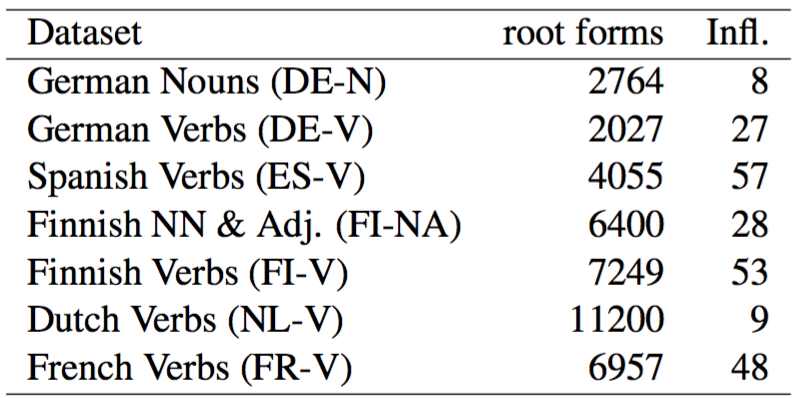
\includegraphics[width=.5\linewidth]{data_inflections}
\end{center}
\end{figure}
\vfill
The languages above were tested with the data published by:
\begin{itemize}
\item {[}Durrett and DeNero 2013{]} containing inflections for German, Finnish and Spanish.
\item {[}Nicolai et al., 2015{]} adding dutch and french to this dataset.
\item The development and test sets contain about 200 inflection tables each.
\end{itemize}

\vfill
{\footnotesize {[}Durrett and DeNero 2013{]}: Supervised learning of complete morphological paradigms. In Proc. of NAACL.}\\
{\footnotesize {[}Nicolai et al., 2015{]}: Inflection generation as discriminative string transduction. In Proc. of NAACL}\\

%%%%%%%%%%%%%%%%%%%%%%%%%%%%%%%%%%%%%%%%%%%%%%%%%%%%%%%%%%%%%%%%%%%%%%%%%%%%%%%%
\NewPage\headline{Application 3: Evaluation}

\begin{figure}[H]
\begin{center}
  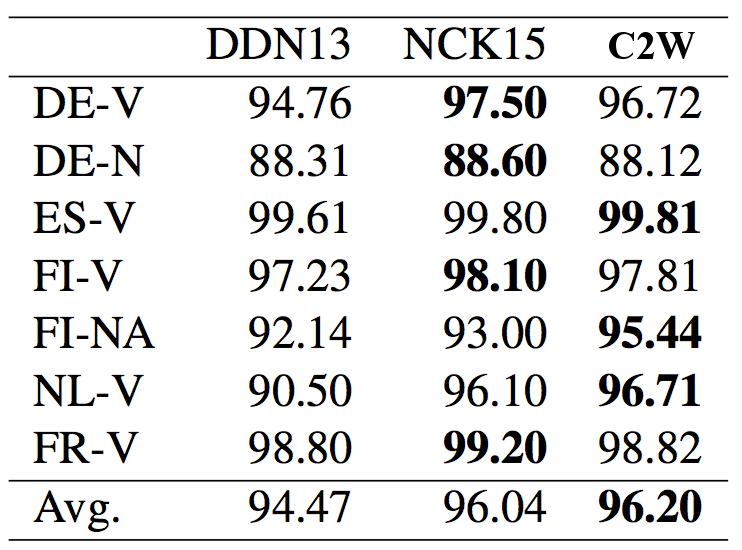
\includegraphics[width=.4\linewidth]{evaluation_inflections}
\end{center}
\end{figure}
\begin{itemize}
\item The results are comparable or better than other approaches.
\item On average the results are better.
\item No feature engineering necessary.
\end{itemize}


%%%%%%%%%%%%%%%%%%%%%%%%%%%%%%%%%%%%%%%%%%%%%%%%%%%%%%%%%%%%%%%%%%%%%%%%%%%%%%%%
\NewPage\headline{Summary}

\vfill
\begin{itemize}
\item Generating word embeddings by composing character representations, works usually just as well
      as approaches using word lookup tables.
\item Lexical features can be learned automatically, manual feature engineering can be avoided
\item In combination with caching of frequently used words, the performance is comparable to models based on word lookup tables.
\item Models scale better with larger vocabularies and are able to deal with open vocabularies.
\end{itemize}
\vfill

\end{document}
